\documentclass{article}
\usepackage[left=1.9cm, right=1.9cm, top=2cm, bottom=2.5cm]{geometry}
\usepackage{graphicx}
\usepackage{caption}
\usepackage{subcaption}


\title{REINFORCEMENT LEARNING WITH
PROBABILISTICALLY COMPLETE EXPLORATION}
\author{ }
\date{December 2023}

\begin{document}

\maketitle
\begin{abstract}
    Balancing exploration and exploitation remains a key challenge in reinforcement
learning (RL). State-of-the-art RL algorithms suffer from high sample complexity,
particularly in the sparse reward case, where they can do no better than to explore in
all directions until the first positive rewards are found. To mitigate this, we propose
Rapidly Randomly-exploring Reinforcement Learning (R3L). We formulate exploration as a search problem and leverage widely-used planning algorithms such as
Rapidly-exploring Random Tree (RRT) to find initial solutions. These solutions are
used as demonstrations to initialize a policy, then refined by a generic RL algorithm,
leading to faster and more stable convergence. We provide theoretical guarantees
of R3L exploration finding successful solutions, as well as bounds for its sampling
complexity. We experimentally demonstrate the method outperforms classic and
intrinsic exploration techniques, requiring only a fraction of exploration samples
and achieving better asymptotic performance.

\end{abstract}

\section{Introduction}
Reinforcement Learning (RL) studies how agents can learn a desired behaviour by simply using interactions with an environment and a reinforcement signal. Central to RL is the long-standing problem
of balancing exploration and exploitation. Agents must first sufficiently explore the environment to
identify high-reward behaviours, before this knowledge can be exploited and refined to maximize
long-term rewards. Many recent RL successes have been obtained by relying on well-formed reward
signals, that provide rich gradient information to guide policy learning. However, designing such
informative rewards is challenging, and rewards are often highly specific to the particular task being
solved. Sparse rewards, which carry little or no information besides binary success or failure, are
much easier to design. This simplicity comes at a cost; most rewards are identical, so that there is
little gradient information to guide policy learning. In this setting, the sample complexity of simple
exploration strategies was shown to grow exponentially with state dimension in some cases (Osband
et al., 2016b). Intuition behind this phenomenon can be gained by inspecting Figure 1a: exploration
in regions where the return surface is flat leads to a random walk type search. This inefficient search
continues until non-zero gradients are found, which can then be followed to a local optimum.
Planning algorithms can achieve much better exploration performance than random walk by taking
search history into account (Lavalle, 1998). These techniques are also often guaranteed to find a
solution in finite time if one exists (Karaman & Frazzoli, 2011). In order to leverage the advantages
of these methods, we formulate RL exploration as a planning problem in the state space. Solutions
found by search algorithms are then used as demonstrations for RL algorithms, initializing them in
regions of policy parameter space where the return surface is not flat. Figure 1b shows the importance
of such good initialization; surface gradients can be followed, which greatly facilitates learning.
This paper brings the following contributions. We first formulate RL exploration as a planning
problem. This yields a simple and effective method for automatically generating demonstrations
without the need for an external expert, solving the planning problem by adapting the classic
\begin{figure}
\begin{subfigure}[b]{0.3\textwidth}
    \centering
    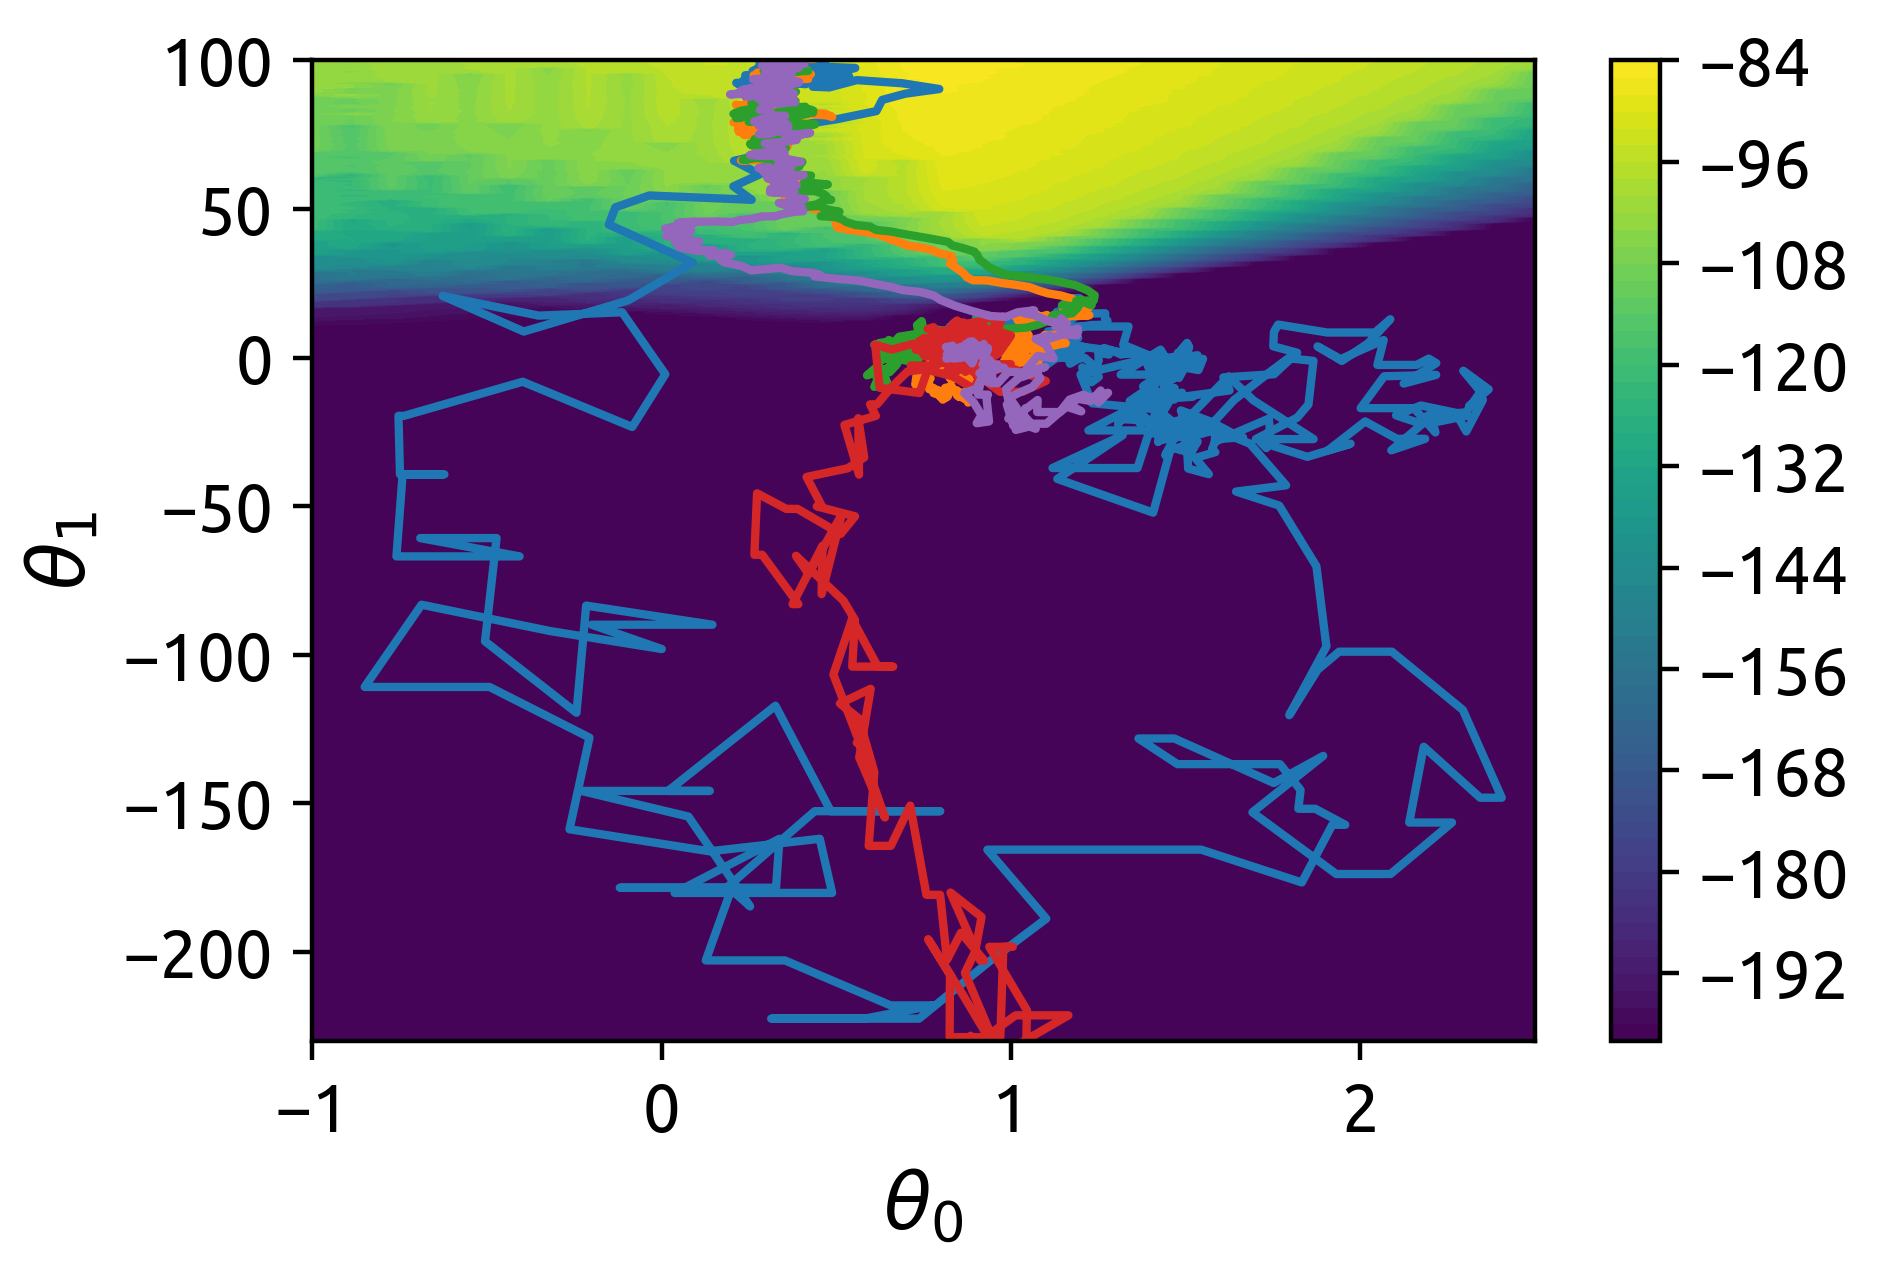
\includegraphics[width=\textwidth]{img-1.png}
    \caption{$\theta _0$}
    \label{fig1}
\end{subfigure}
\begin{subfigure}[b]{0.3\textwidth}
    \centering
    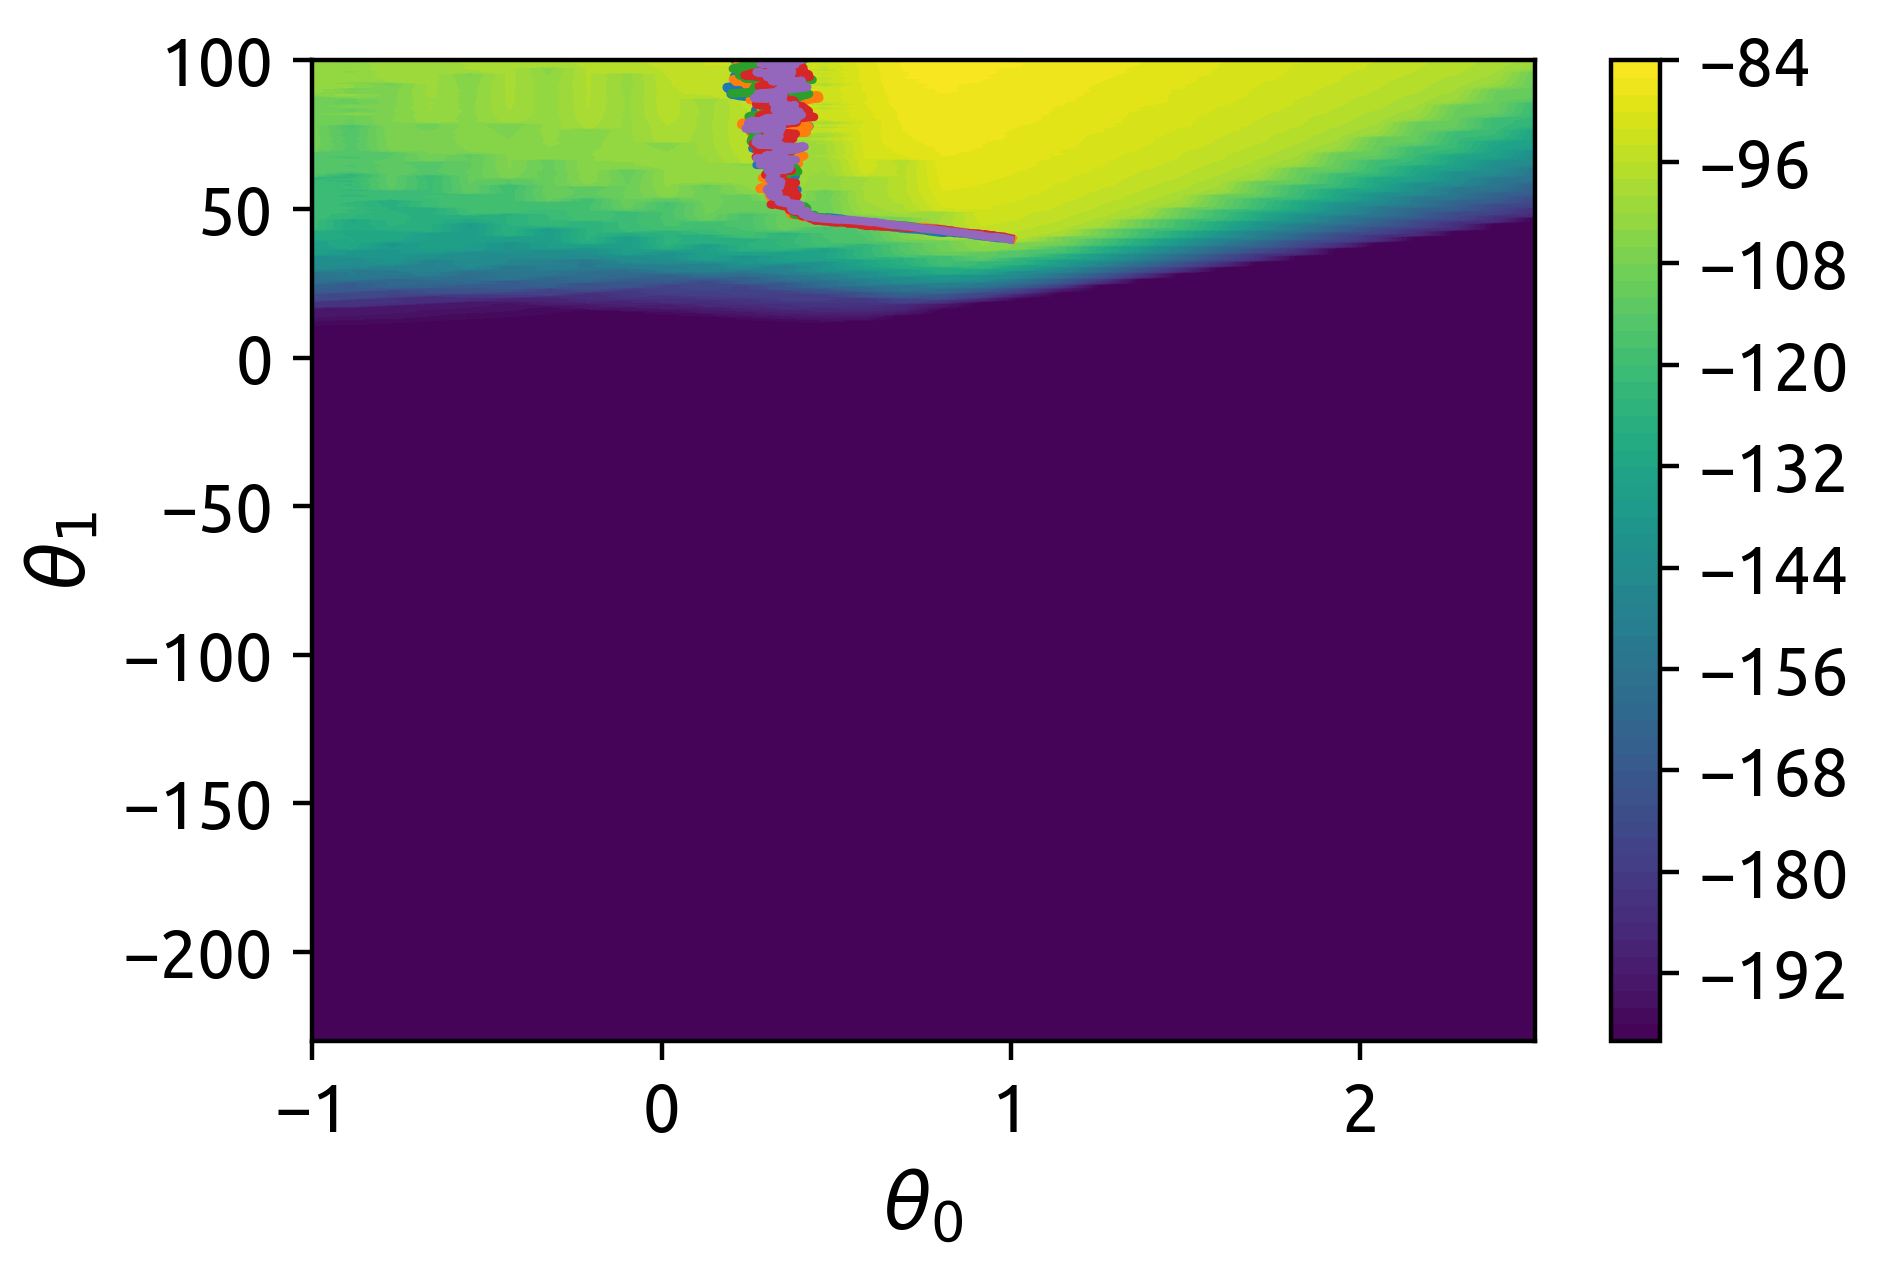
\includegraphics[width=\textwidth]{img-3.png}
    \caption{$\theta _0$}
    \label{fig2}
\end{subfigure}
\end{figure}

Figure 1: Expected returns achieved by linear policy with 2 parameters on Sparse MountainCar
domain (background). Gradient is 0 in the dark blue area. Trajectories show the evolution of policy
parameters over 1000 iterations of TRPO, with 5 random seeds. Same colors indicate the same
random seeds. \ref{fig1} Random-walk type behaviour observed when parameters are initialized using
Glorot initialization (Glorot \& Bengio, 2010). \ref{fig2} Convergence observed when parameters are
initialized in a region with gradients (1, 40).
Rapidly-exploring Random Tree algorithm (RRT) (Kuffner & LaValle, 2000). The demonstrations
are then used to initialize an RL policy, which can be refined with a classic RL method such
as TRPO (Schulman et al., 2015). We call the proposed method Rapidly Randomly-exploring
Reinforcement Learning (R3L)1
, provide theoretical guarantees for finding successful solutions
and derive bounds for its sampling complexity. Experimentally, we demonstrate R3L improves
exploration and outperforms classic and recent exploration techniques, and requires only a fraction of
the samples while achieving better asymptotic performance. Lastly, we show that R3L lowers the
variance of policy gradient methods such as TRPO, and verify that initializing policies in regions
with rich gradient information makes them less sensitive to initial conditions and random seed.
The paper is structured as follows: Section 2 analyzes the limitations of classic RL exploration.
Section 3 describes R3L and provides theoretical exploration guarantees. Related work is discussed in
Section 4, followed by experimental results and comments in Section 5. Finally, Section 6 concludes
and gives directions for future work.

\section{ SPARSE-REWARD RL AS RANDOM WALK}
Many recent RL methods are based on a policy gradient optimization scheme. This approach
optimizes policy parameters $\theta$ with gradient descent, using a loss function ${\mathcal{L}}(\theta)$  (e.g. expected return)
and gradient $g(\theta)\,\equiv\,\nabla_{\theta}Z(\theta), $. Since computing  ${\mathcal{L}}(\theta)$ exactly is intractable, it is common to use
unbiased empirical estimators ${\hat{L}}(\theta) $  and ${\hat{g}}(\theta) $ , estimated from samples acquired by executing the policy.
Optimization of θ then follows the common \textit{stochastic gradient descent} t (SGD) update-rule (Bottou,
2010; Robbins \& Monro, 1951): 
$
\theta_{n+1}=\theta_{n}-\epsilon{\hat{g}}\,(\theta_{n}) 
$ where E is the learning rate

The SGD update rule defines a discrete-time stochastic process (Mandt et al., 2017). Note that  ${\hat{g}} $ is the mean of $n _mb$ b i.i.d. samples. Following the central limit theorem, the distribution over ${\hat{g}} $ is
approximately 
$$
{\hat{g}}(\theta)\sim{\mathcal{N}}(g(\theta),{\frac{1}{n_{m a}}}C(\theta)) 
$$
meaning  ${\hat{g}} $ is an unbiased estimator of g with covariance ${\frac{1}{n_{m a}}}C(\theta))$ Consequently, the update rule can be rewritten as (Mandt et al., 2017):

$$
\theta_{n+1}=\theta_{n}-\epsilon g(\theta_{n})+\frac{\epsilon}{n_{m b}}B\Delta W,\qquad\Delta W\sim\mathcal{N}(0,\bar{1}). 
$$
Here we assume that  $C(\theta)=C,$ i.e. approximately constant w.r.t. ${\boldsymbol{\theta}}.$ and factorizes as $C=B B^{T}$ 
.
SGD is efficient for high-dimensional problems as it offers almost dimension independent convergence
rates (Nesterov, 2018). However, SGD requires non-zero gradients to guide the search towards the
optimum $\theta^{*}$ , i.e. $|g(\theta)|>\epsilon_{\alpha},\forall\theta\ne\theta^{*}$  $\epsilon_{\mathcal{I}}\in\mathbb{R}$ In the case of sparse-reward RL problems, such as in Figure l, much of the loss surfaceis flat. This leadsto inefficient exploration of parameter space $\mathbf{\Theta}(0)$ as the drift component in Eq. (1) $g\approx0.$  turning the SGD to a random walk in $\Theta\colon\Delta\theta={\frac{e}{n_{m b}}}B\Delta W$ Random walk is guaranteed to wander to infinity when dimensionality $d\sigma\geq3$ (Polya, 1921; Kakutani, l944). However, the probability of it reaching a desired region in $\mathbf{\Lambda}(\mathbf{\alpha})$  e.g. where $a\neq0$ , depends
able mpact of learning local policy ${\boldsymbol{\pi}}_{l}$ and biasing search towards $\mathcal{F}_{g o a l}$ with probability $\ p_{g}\,$ on R3L exploration. Results show the mean and standard deviation of successful trajectory length $\left|{\boldsymbol{\tau}}\right|$ and number of timesteps required., computed over 2O runs


Accelerating RL by learning from demonstration was investigated in Niekum et al. (2015); Bojarski
et al. (2016); Torabi et al. (2018). However, these techniques rely on user-generated demonstrations or a-priori knowledge of environment parameters. In contrast, R3L automatically generates
demonstrations, with no need of an external expert.

\section{EXPERIMENTS}
In this section, we investigate (i) how learning a local policy πl and biasing search towards Fgoal with
probability pg affects R3L exploration, (ii) whether separating exploration from policy refinement
is a viable and robust methodology in RL, (iii) whether R3L reduces the number of exploration
samples needed to find good policies, compared with methods using classic and intrinsic exploration,
and (iv) how R3L exploration can reduce the variance associated with policy gradient methods.
All experiments make use of the Garage (Duan et al., 2016) and Gym (Brockman et al., 2016)
frameworks. The experimental setup features the following tasks with sparse rewards: Cartpole
SWingup $(S\subseteq\mathbb{R}^{4},{\mathcal{A}}\subseteq\mathbb{R})$ MountainCar $(S\subseteq\mathbb{R}^{2},{\mathcal{A}}\subseteq\mathbb{R})$ Acrobot $(S\subseteq\mathbb{R}^{4},{\mathcal{A}}\subseteq\mathbb{R})$ Pendulun (S GR,A C R) Reacherc $(S\subseteq\mathbb{R}^{6},{\mathcal{A}}\subseteq\mathbb{R}^{2})$ Fetch Reach c $\mathbb{S}\subseteq\mathbb{R}^{13},{\mathcal{A}}\subseteq\mathbb{R}^{4}.$ , and Hand Reacl $(S\subseteq\mathbb{R}^{78},A\subseteq\mathbb{R}^{20})$ The exact environment and reward definitions are described in Appendix S3
\textbf{R3L exploration analysis} We first analyze the exploration performance of R3L in a limited set of
RL environments, to determine the impact that learning policy πl has on exploration speed. We also
investigate whether R3L exploration is viable in environments where no goal information is available.
Table 1 shows the results of this analysis. Learning πl seems to greatly decrease the number of
exploration timesteps needed on most environments. However, it significantly increases the number
of timesteps on the acrobot and reacher environments. Results also suggest that learning πl helps
R3L to find shorter trajectories on the same environments, which is a desirable property in many RL
problems. Biasing R3L exploration towards the goal set Fgoal helps finding successful trajectories
faster, as well as reducing their length. However, R3L exploration without goal bias is still viable in
all cases. Although goal information is not given in the classic MDP framework, it is often available
in real-world problems and can be easily utilized by R3L. Lastly, successful trajectory lengths have
low variance, which suggests R3L finds consistent solutions.
Comparison to classic and intrinsic exploration on RL benchmarks We examine the rates at
which R3L learns to solve several RL benchmarks, and compare them with state-of-the-art RL
algorithms. Performance is measured in terms of undiscounted returns and aggregated over 10
random seeds, sampled at random for each environment. We focus on domains with sparse rewards,
which are notoriously difficult to explore for traditional RL methods. Our experiments focus on the
widely-used methods TRPO (Schulman et al., 2015) and DDPG (Lillicrap et al., 2015). R3L-TRPO
and R3L-DDPG are compared to the baseline algorithms with Gaussian action noise. As an additional
baseline we include VIME-TRPO (Houthooft et al., 2016). VIME is an exploration strategy based on
maximizing information gain about the agent’s belief of the environment dynamics. It is included to
show that R3L can improve on state-of-the-art exploration methods as well as naive ones, even though
the return surface for VIME-TRPO is no longer flat, unlike Figure 1. The exact experimental setup is
described in Appendix S3.2. The R3L exploration phase is first run to generate training trajectories
for all environments. The number of environment interactions during this phase is accounted for in
the results, displayed as an offset with a vertical dashed black line. The average performance achieved
7
outperforms classic and intrinsic exploration techniques, requiring only a fraction of exploration
samples and achieving better asymptotic performance.
As future work, R3L could be extended to real-world problems by leveraging recent advances on
bridging the gap between simulation and reality (Peng et al., 2018). Respecting Assumption 2, a
policy would first be trained on a simulator and then transferred to the real-world. Exploration in
high-dimensional tasks is also challenging as stated in Theorem 3 and confirmed experimentally
by increased R3L exploration timesteps. Exploiting external prior knowledge and/or the structure
of the problem can benefit exploration in high-dimensional tasks, and help make R3L practical for
problems such as Atari games. Lastly, recent advances in RRT (Chiang et al., 2019) and learning
from demonstration (Torabi et al., 2018) could also improve R3L.
\end{document}
